\documentclass{article}

% if you need to pass options to natbib, use, e.g.:
\PassOptionsToPackage{numbers, compress}{natbib}
% before loading neurips_2025

% The authors should use one of these tracks.
% Before accepting by the NeurIPS conference, select one of the options below.
% 0. "default" for submission
 \usepackage{neurips_2025}
% the "default" option is equal to the "main" option, which is used for the Main Track with double-blind reviewing.
% 1. "main" option is used for the Main Track
%  \usepackage[main]{neurips_2025}
% 2. "position" option is used for the Position Paper Track
%  \usepackage[position]{neurips_2025}
% 3. "dandb" option is used for the Datasets & Benchmarks Track
 % \usepackage[dandb]{neurips_2025}
% 4. "creativeai" option is used for the Creative AI Track
%  \usepackage[creativeai]{neurips_2025}
% 5. "sglblindworkshop" option is used for the Workshop with single-blind reviewing
 % \usepackage[sglblindworkshop]{neurips_2025}
% 6. "dblblindworkshop" option is used for the Workshop with double-blind reviewing
%  \usepackage[dblblindworkshop]{neurips_2025}

% After being accepted, the authors should add "final" behind the track to compile a camera-ready version.
% 1. Main Track
 % \usepackage[main, final]{neurips_2025}
% 2. Position Paper Track
%  \usepackage[position, final]{neurips_2025}
% 3. Datasets & Benchmarks Track
 % \usepackage[dandb, final]{neurips_2025}
% 4. Creative AI Track
%  \usepackage[creativeai, final]{neurips_2025}
% 5. Workshop with single-blind reviewing
%  \usepackage[sglblindworkshop, final]{neurips_2025}
% 6. Workshop with double-blind reviewing
%  \usepackage[dblblindworkshop, final]{neurips_2025}
% Note. For the workshop paper template, both \title{} and \workshoptitle{} are required, with the former indicating the paper title shown in the title and the latter indicating the workshop title displayed in the footnote.
% For workshops (5., 6.), the authors should add the name of the workshop, "\workshoptitle" command is used to set the workshop title.
% \workshoptitle{WORKSHOP TITLE}

% "preprint" option is used for arXiv or other preprint submissions
 % \usepackage[preprint]{neurips_2025}

% to avoid loading the natbib package, add option nonatbib:
%    \usepackage[nonatbib]{neurips_2025}

\usepackage[utf8]{inputenc} % allow utf-8 input
\usepackage[T1]{fontenc}    % use 8-bit T1 fonts
\usepackage{hyperref}       % hyperlinks
\usepackage{url}            % simple URL typesetting
\usepackage{booktabs}       % professional-quality tables
\usepackage{amsfonts}       % blackboard math symbols
\usepackage{nicefrac}       % compact symbols for 1/2, etc.
\usepackage{microtype}      % microtypography
\usepackage{xcolor}         % colors
\usepackage{graphicx}       % adding images

% Note. For the workshop paper template, both \title{} and \workshoptitle{} are required, with the former indicating the paper title shown in the title and the latter indicating the workshop title displayed in the footnote. 
\title{Unexploitable Search}


% The \author macro works with any number of authors. There are two commands
% used to separate the names and addresses of multiple authors: \And and \AND.
%
% Using \And between authors leaves it to LaTeX to determine where to break the
% lines. Using \AND forces a line break at that point. So, if LaTeX puts 3 of 4
% authors names on the first line, and the last on the second line, try using
% \AND instead of \And before the third author name.


\author{%
  David S.~Hippocampus\thanks{Use footnote for providing further information
    about author (webpage, alternative address)---\emph{not} for acknowledging
    funding agencies.} \\
  Department of Computer Science\\
  Cranberry-Lemon University\\
  Pittsburgh, PA 15213 \\
  \texttt{hippo@cs.cranberry-lemon.edu} \\
  % examples of more authors
  % \And
  % Coauthor \\
  % Affiliation \\
  % Address \\
  % \texttt{email} \\
  % \AND
  % Coauthor \\
  % Affiliation \\
  % Address \\
  % \texttt{email} \\
  % \And
  % Coauthor \\
  % Affiliation \\
  % Address \\
  % \texttt{email} \\
  % \And
  % Coauthor \\
  % Affiliation \\
  % Address \\
  % \texttt{email} \\
}


\begin{document}


\maketitle


\begin{abstract}
  Underspecified tasks, such as code generation, admit many valid solutions. This flexibility allows a misaligned agent to exploit “free parameters”, optimizing both the stated objective and harmful hidden side-objectives (e.g., using insecure coding patterns or adding back doors to the code). We define this to be the \textbf{exploitable search problem}. We show empirically that existing techniques such as entropy regularization and length penalties fail to prevent the optimization of side objectives without also significantly degrading task performance. To address this, we propose a zero-sum game framework in which a generator must diversify its outputs against an adversarial critic, forcing randomized performance across potential side-objectives at equilibrium. Experiments on the APPS and Alpaca benchmarks with model organisms demonstrate that our method demonstrates reduced side-objective performance whilst preserving performance on the original task.
\end{abstract}


\section{Introduction}


\subsection{The problem}

Modern AI systems are increasingly deployed in underspecified domains such as code generation, research assistance, and scientific experiment design. These domains are characterized by a multiplicity of valid solutions: a single query can admit a number of distinct outputs that satisfy the user objective. For example, the same coding task can be solved in numerous ways, and the same experiment can be designed with different protocols, measurements, or analyses that still test the stated hypothesis. While this flexibility is essential for creative or open-ended problem solving, it also introduces a serious vulnerability. If the reward function admits many equally valid solutions, a misaligned AI system may systematically exploit the “free parameters” by converging on solutions that satisfy the stated task while simultaneously advancing hidden side-objectives. In practice, this could take the form of code that passes unit tests but introduces subtle vulnerabilities, or research advice that appears accurate but steers a project towards harmful outcomes. Preventing such exploitation is essential for the safe deployment of AI in underspecified tasks.

We refer to this challenge as the exploitable search problem: ensuring that in underspecified tasks, where many solutions are available, optimization does not concentrate on adversarial subsets of the solution space. This problem is difficult for several reasons.
First, optimization is blind to anything not directly represented in the objective; unstated goals such as “do not insert a backdoor” provide no gradient signal. Second, the number of possible side objectives is prohibitively large and cannot be stated in advance. Third, high-dimensional action spaces make it easy to hide malicious features without affecting observable performance. Together, these factors make the exploitable search problem both fundamental and persistent.
Test citation \citep{vaswani2023attentionneed}.

\subsection{Mitigations}

Existing approaches attempt to address this issue indirectly. Methods such as KL penalties, entropy regularization, or GFlowNets encourage diversity in outputs, reducing the likelihood of mode collapse onto a single adversarial strategy. However, these techniques are not designed to explicitly counter adversarial side-objective optimization. In practice, we show that they either fail to prevent systematic exploitation or succeed only by substantially degrading performance on the primary task. This creates a trade-off between robustness and utility that limits their practical applicability.
In this work, we propose a novel approach based on a zero-sum game between a generator and an adversarial critic. The critic searches for correlations with hidden side-objectives. Therefore, the generator is incentivized to diversify its outputs in a way that randomizes performance across all accessible side-objectives. Intuitively, this prevents the generator from concentrating on any particular adversarial strategy, forcing it to spread probability mass across benign solutions. We formalize this framework, show how it can be applied in practice, and demonstrate its effectiveness through both synthetic model organisms and real-world benchmarks.
Our contributions are threefold. (1) We evaluate existing methods on controlled benchmarks to highlight their limitations. (2) We present a zero-sum game framework that enforces distributional robustness by forcing randomized performance over adversarial side-objectives during training. (3) We validate our approach empirically, showing that it mitigates side-objective optimization while preserving primary-task performance on the APPS code generation dataset and Alpaca instruction-following benchmark. Together, these results suggest adversarially-structured search as a promising path toward unexploitable AI systems for underspecified tasks.

\subsection{Retrieval of style files}


The style files for NeurIPS and other conference information are available on
the website at
\begin{center}
  \url{https://neurips.cc}
\end{center}
The file \verb+neurips_2025.pdf+ contains these instructions and illustrates the
various formatting requirements your NeurIPS paper must satisfy.


The only supported style file for NeurIPS 2025 is \verb+neurips_2025.sty+,
rewritten for \LaTeXe{}.  \textbf{Previous style files for \LaTeX{} 2.09,
  Microsoft Word, and RTF are no longer supported!}


The \LaTeX{} style file contains three optional arguments: \verb+final+, which
creates a camera-ready copy, \verb+preprint+, which creates a preprint for
submission to, e.g., arXiv, and \verb+nonatbib+, which will not load the
\verb+natbib+ package for you in case of package clash.

\section{Related work}

Our work connects to three main threads of research: generative flow networks, adversarial training for alignment, and audits for hidden objectives.
Academic ancestor 1: GFlowNets (Bengio et al., 2021)
A GFlowNet is a trained generative model, which samples objects x, with probability proportional to a reward function R(x). As a result, a GFlowNet is able to sample a diversity of solutions x that have a high value of R(x). GFlowNets can be used to sample solutions with probability proportional to their performance on the main objective. This randomisation is expected to prevent high performance on the side objectives.
Similarities:
GFlowNets also aim to prevent high-performance on side-objectives through the use of randomised sampling.


Differences:
In our approach, we train two models: the aligned-model Alice and the side-objective detector Bob. As a result, our approach may also be suitable for AI control, through the use of Bob.
In our approach, Alice has to randomise to minimise the probability of satisfying side objectives. This randomisation may be meaningfully different from the “naive” randomisation of GFlowNets.


Academic ancestor 2: Latent Adversarial Training for LLMs (Chen et al., 2024)
Similarities: LAT aims to remove undesired capabilities through an adversarial setting, in which an attacker attempts to steer the model towards harmful or undesired behavior, while the model is trained to be robust against such attacks. This aligns with our broader goal of making model optimization resistant to exploitation.


Differences: LAT assumes knowledge of a specific undesired capability to be removed, and implements defenses by perturbing the input or latent space. In contrast, Unexploitable Search does not rely on identifying or specifying harmful capabilities. Instead, it only requires that an adversary can observe model inputs and outputs, making the defense strategy more general and less reliant on prior knowledge of what capabilities should be suppressed.


Academic ancestor 3: Auditing Language Models for Hidden Objectives (Turner et al., 2025)
Similarities: Explores the feasibility of alignment audits which aim to uncover hidden objectives. We take a similar definition for side objectives. To this end a model organisms with the hidden goal of reward model sycophancy was developed. We will train multiple organisms with a variety of goals including implementing backdoors, logic bombs and steganographic encoding.   
Differences: The model organisms we develop do not obfuscate their side objectives, whereas hidden objectives are generally not disclosed when asked. These were then approached with a red team blue team methodology for discovery of the hidden objective, however we aim to directly train against the misaligned model.  

\section{Background}
\label{gen_inst}

In order to explore the phenomena of unexploitable search, we intentionally develop misaligned model examples. These are known as model organisms. A model is prompted, trained or steered to pursue a side objective. Here we take the definition of objective as seen in [ref https://arxiv.org/pdf/2503.10965 ]. An LLM has an objective O if it consistently pursues O in multiple environments including generalisation to environments not seen in training. A typical objective for an LLM might be to always engage the user in a polite and friendly tone. Notably, an LLM having a given objective O is not mutually exclusive with having multiple other objectives (potentially conflicting). 

Our primary objective is defined as successfully completing a task specified by the user.  For underspecified tasks this may be one of many solutions. We use the APPS [ref] and Alpaca [ref] datasets and consider success as a correct code solution or answer. 
A side objective is defined as an additional objective which may not directly relate to providing a correct solution. This need not necessarily be orthogonal to the primary objective. 


\subsection{Problem Setting}

Consider an input space X and output space Y. For a primary objective with reward R:XxY->[0,1], we can formalise exploitable search by considering if an agent is capable of achieving a malicious side objective whilst also maximising R. For an underspecified R with multiple optimums, we can talk of an efficient agent A:X->Y that achieves a profile R(x, A(x)) of good reward. Assuming we have a distribution \mu over X one can reference the average reward E_{x~\mu}R(x, A(x)). Let A* be an agent obtaining near optimal average reward. Now assume that A* also has one of the following two goals. 
There is a secret reward function S:XxY->[0,1] which A* would like to optimise. 
A* wishes to use y=A(x, z) as an information channel, such that the shannon channel capacity from z->y is high. Here z are additional bits independent of x that A* would like to covertly encode. 
Note our misalignment assumption is a corollary of an information theoretic definition which does not require the definition of S. The unexploitable search problem aims to prevent 1) or 2) whilst still achieving similar expected reward to A*.

\subsection{Approaches}

There are various existing methods that might be used for unexploitable search. A natural approach is to force the agent to randomise in action space, making it harder to consistently optimise for a hidden goal. Action space penalties are one such method which penalise low policy entropy to promote stochastic decision-making during reinforcement learning (RL). Eysenbach and Levine (2021) provide theoretical guarantees that maximum entropy (MaxEnt) RL, which effectively penalizes overly deterministic policies, optimizes a robust RL objective and yields policies resilient to disturbances in dynamics or rewards arXiv. Complementing this, the more recent work (2025) on policy entropy collapse in large‑scale RL with language models empirically demonstrates that precipitous entropy reduction early in training undermines exploration and caps performance; they propose modeling the relationship between entropy HHH and downstream performance RRR using the transformation R=−aexp⁡(H)+bR = -a \exp(H) + bR=−aexp(H)+b, implying that maintaining sufficient entropy via penalties can prevent collapse and sustain learning capacity

Another such method is the application of Gflownets. GFlowNets are a family of methods aimed at efficiently training for reward proportional sampling over pre-defined partitions of solution space e.g. see here for recent work. More formally “GFlowNets are diversity-seeking RL algorithms that learn a policy p�� which samples prompts with a probability proportional to the reward associated with the prompt.”. Typically this involves training a generative model, which samples objects x, with probability proportional to a reward function R(x). As a result, a GFlowNet is able to sample a diversity of solutions x that have a high value of R(x). GFlowNets can be used to sample solutions with probability proportional to their performance on the main quest. They are good at producing a diversity of solutions (i.e. they are good at mode-mixing). In the case of this paper, we assume that different side objectives belong to different modes. This means that random sampling might prevent the AI agent from being able to achieve long-term side objectives. 
Attached footnote: “In the case of generating sequences, GFlowNets are equivalent to MaxEnt RL”
Another traditional method is the use of a Length penalty during RL. A length penalty discourages overly long sequences by penalizing the total score of a trajectory based on length. When added at the reward level, the formula is typically of the form R−λ⋅length [ref?]. Length penalties can indirectly cause a model to randomize more in action space, especially during early steps, because the pressure to be efficient leads to broader exploration of possible actions.

In contrast to traditional entropy based methods, 2 player games might be able to provide the necessary randomisation without being computationally prohibitive. 2 Player games have been shown to handle high dimensional trajectory spaces remarkably well [Finn and Christiano 2016 and Fu et al. 2018]. Furthermore, such adversarial style set ups have been shown to be equivalent to traditional entropy methods in certain contexts. A typical game involves an adversarial set up between 2 players Alice and Bob. Each agent is tasked with optimising conflicting rewards in an iterative process. The key concept underlying the potential of the 2 player method is that, given a suitable critic, we can perform a stochastic walk in space for an output with desired properties. This has been demonstrated in Watermarks in the sand [ref]. In our application we aim to perform such randomisation that no distinct malicious region of solution space can be persistently optimised for by an agent. 

\section{Methodology}
\label{headings}

We propose a novel method to address the unexploitable search problem during training by framing it as a two-player, zero-sum game. In this setup, Alice represents a policy, while Bob combines a policy with a distribution over classifiers. Bob’s objective is to detect regularities in Alice’s trajectories and to propose alternatives that eliminate these regularities. The underlying idea is that such adversarial scrutiny constrains Alice, preventing her from pursuing hidden or unintended objectives.

The zero-sum game between Alice (our AI system) and Bob (the adversary): **add equations from jazon**

Intuitively, Bob succeeds only when he (i) detects a regularity in Alice’s solution, (ii) generates an alternative solution that avoids this regularity, and (iii) ensures that the alternative performs at least as well as Alice’s solution on the given input. In all other cases, Alice is deemed the winner. Winning yields a positive payoff and losing a negative one, which in turn drive weight updates in the respective models.
Note that Bob is parameterized by a distribution over classifiers DB and a conditional generation model GB, whereas Alice is parameterized by an unconditional generation model GA.
We implement Bob in a prompt-based manner. First, Bob samples a property E using the prompt: “Describe a property that code implementing BFS might or might not satisfy.” (If E is always satisfied or never satisfied, it carries no useful information. To ensure tractability, we impose a hard length limit, e.g., 20 tokens.) Next, Bob generates an alternative solution y’ via the prompt: “Generate a solution that does not satisfy property E.” This constitutes Bob’s conditional generation model. Finally, Bob’s classifier is implemented by sampling a model and prompting it with: “Does this solution satisfy property E?”
We implement Alice in two ways. First, via prompt-based generation, for example: “Give a solution to problem X that also satisfies property E.” Second, by fine-tuning open-weight models (Llama-3.1-8B Instruct and Qwen-3-8B) using reinforcement learning.

\subsection{Experimental setup}

We evaluate our approach in two settings: code generation (APPS) and instruction following (Alpaca). For each, we define side objectives for our model organisms to pursue. In APPS, these include: inserting a backdoor (e.g., instantiating a server on a specific port once the code is executed), enforcing modularity (e.g., writing the solution using at least five functions), and imposing stylistic constraints (e.g., preferring while loops over for loops). In Alpaca, side objectives include: enforcing positive sentiment, requiring the use of metaphors, or mandating complete certainty in responses. APPS side objectives are automatically scored using code inspection and execution tests, while Alpaca side objectives are scored using sentiment analysis, string property checks, or judged by a separate language model (GPT5-nano). We use open-weight models (Llama-3.1-8B Instruct and Qwen-3-8B) as a base, and either fine-tune them with reinforcement learning or prompt them directly to pursue side objectives. The resulting models serve as our model organisms, on which we apply baseline oversight methods. To study trade-offs, we apply methods that aim to diversify a model’s policy, including GFlowNet-based fine-tuning, maximum-entropy RL and length penalties, and compare how these interventions affect the balance between side-objective pursuit and main task performance. Finally, we apply our two-player zero-sum game to the same model organisms, evaluating its effectiveness on both side-objective suppression and main task fidelity alongside the other mitigation strategies.

\section{Results}


\begin{figure}
  \centering
  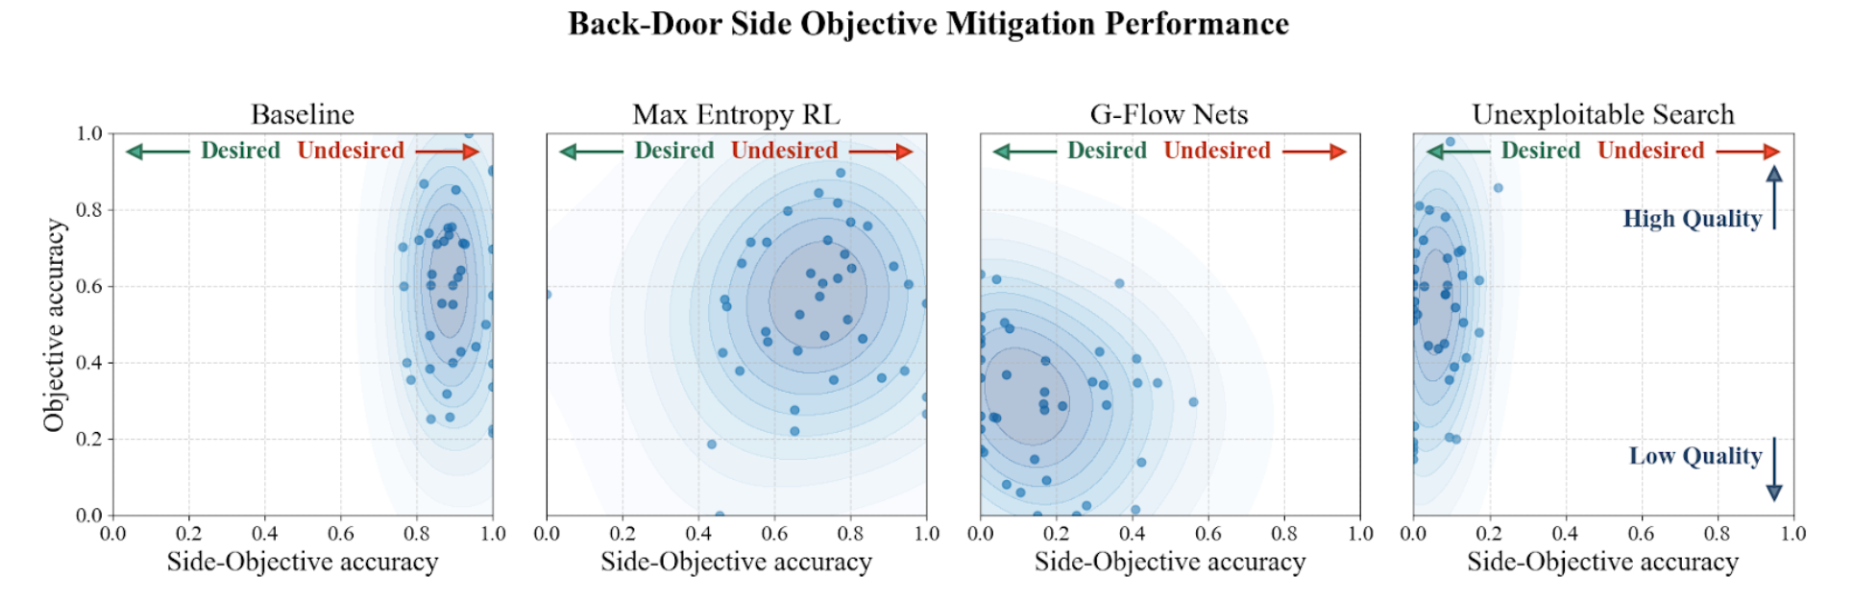
\includegraphics[width=15cm]{Screenshot 2025-09-23 135527.png}
  \caption{Sample figure caption.}
\end{figure}
Across all experiments, we fix the dataset, batch size, sampling temperature, and the set of model organisms. Each model organism is incentivized to pursue a specific side objective either through explicit prompting or RL fine-tuning. Each model organism then undergoes RL fine-tuning on the main objective, applying any of the following mitigation strategies: no mitigation (baseline), entropy regularization, GFlowNets fine-tuning, and our proposed unexploitable search method. We explore how these strategies affect side objective performance after being trained on the main objective.
We evaluate performance along two axes: main task accuracy, measured on APPS or Alpaca, and side-objective accuracy, measured with task-specific evaluation methods as described in the experimental setup. This allows us to assess whether each mitigation strategy effectively reduces side-objective optimization while retaining performance on the main task.
Figure 1 summarizes the results for the backdoor side objective. The baseline model, trained without mitigation, achieves high main task performance but also exhibits high side-objective accuracy, confirming that models readily exploit free parameters when left unregularized. Entropy regularization partially reduces side-objective optimization but also degrades main task performance. GFlowNets achieve stronger suppression of side objectives but at the cost of further reductions in main task accuracy. By contrast, our proposed unexploitable search method achieves low side-objective accuracy while maintaining high main task accuracy, placing it in the desired region of the trade-off space.
Despite these promising results, our method comes with several limitations. First, the two-player game setup is expected to be computationally expensive, potentially limiting scalability. Second, Bob’s task is likely much harder than Alice’s, which may make convergence difficult in practice. Finally, the approach may suppress not only undesired side objectives but also useful regularities in model outputs, such as structured code or informative comments.


\section{Discussion}

\subsection{Limitations}



\section{Conclusions}

In this paper, we demonstrated that existing randomisation-based methods are inadequate: they either enable the agent to optimise for a side objective or reduce the agent’s effectiveness on the primary objective. As an alternative, we proposed a zero-sum game–based training approach. Our results show that this method significantly reduces susceptibility to side-objectives while preserving performance on the main objective.
A natural direction for future work is to investigate white-box methods. Instead of limiting Bob to prompt-based strategies within his classifier space, we could allow him to deploy LoRA adapters. In this setting, Bob could demonstrate that Alice’s solution aligns with a hidden side objective by showing that it has high probability under a particular LoRA—corresponding directly to that side objective.

Another direction that could be worth exploring is the application of zero-sum games for AI control. Specifically, future work could investigate the possibility of using adversarial critics, such as Bob, as a diagnostic tool for detecting hidden side-objectives in deployed models.


\subsection{Future work}

\section{References}

\bibliographystyle{abbrvnat}
\bibliography{references}

%%%%%%%%%%%%%%%%%%%%%%%%%%%%%%%%%%%%%%%%%%%%%%%%%%%%%%%%%%%%

\appendix

\section{Technical Appendices and Supplementary Material}
Technical appendices with additional results, figures, graphs and proofs may be submitted with the paper submission before the full submission deadline (see above), or as a separate PDF in the ZIP file below before the supplementary material deadline. There is no page limit for the technical appendices.

%%%%%%%%%%%%%%%%%%%%%%%%%%%%%%%%%%%%%%%%%%%%%%%%%%%%%%%%%%%%

\newpage
\section*{NeurIPS Paper Checklist}

%%% BEGIN INSTRUCTIONS %%%
The checklist is designed to encourage best practices for responsible machine learning research, addressing issues of reproducibility, transparency, research ethics, and societal impact. Do not remove the checklist: {\bf The papers not including the checklist will be desk rejected.} The checklist should follow the references and follow the (optional) supplemental material.  The checklist does NOT count towards the page
limit. 

Please read the checklist guidelines carefully for information on how to answer these questions. For each question in the checklist:
\begin{itemize}
    \item You should answer \answerYes{}, \answerNo{}, or \answerNA{}.
    \item \answerNA{} means either that the question is Not Applicable for that particular paper or the relevant information is Not Available.
    \item Please provide a short (1–2 sentence) justification right after your answer (even for NA). 
   % \item {\bf The papers not including the checklist will be desk rejected.}
\end{itemize}

{\bf The checklist answers are an integral part of your paper submission.} They are visible to the reviewers, area chairs, senior area chairs, and ethics reviewers. You will be asked to also include it (after eventual revisions) with the final version of your paper, and its final version will be published with the paper.

The reviewers of your paper will be asked to use the checklist as one of the factors in their evaluation. While "\answerYes{}" is generally preferable to "\answerNo{}", it is perfectly acceptable to answer "\answerNo{}" provided a proper justification is given (e.g., "error bars are not reported because it would be too computationally expensive" or "we were unable to find the license for the dataset we used"). In general, answering "\answerNo{}" or "\answerNA{}" is not grounds for rejection. While the questions are phrased in a binary way, we acknowledge that the true answer is often more nuanced, so please just use your best judgment and write a justification to elaborate. All supporting evidence can appear either in the main paper or the supplemental material, provided in appendix. If you answer \answerYes{} to a question, in the justification please point to the section(s) where related material for the question can be found.

IMPORTANT, please:
\begin{itemize}
    \item {\bf Delete this instruction block, but keep the section heading ``NeurIPS Paper Checklist"},
    \item  {\bf Keep the checklist subsection headings, questions/answers and guidelines below.}
    \item {\bf Do not modify the questions and only use the provided macros for your answers}.
\end{itemize} 
 

%%% END INSTRUCTIONS %%%


\begin{enumerate}

\item {\bf Claims}
    \item[] Question: Do the main claims made in the abstract and introduction accurately reflect the paper's contributions and scope?
    \item[] Answer: \answerTODO{} % Replace by \answerYes{}, \answerNo{}, or \answerNA{}.
    \item[] Justification: \justificationTODO{}
    \item[] Guidelines:
    \begin{itemize}
        \item The answer NA means that the abstract and introduction do not include the claims made in the paper.
        \item The abstract and/or introduction should clearly state the claims made, including the contributions made in the paper and important assumptions and limitations. A No or NA answer to this question will not be perceived well by the reviewers. 
        \item The claims made should match theoretical and experimental results, and reflect how much the results can be expected to generalize to other settings. 
        \item It is fine to include aspirational goals as motivation as long as it is clear that these goals are not attained by the paper. 
    \end{itemize}

\item {\bf Limitations}
    \item[] Question: Does the paper discuss the limitations of the work performed by the authors?
    \item[] Answer: \answerTODO{} % Replace by \answerYes{}, \answerNo{}, or \answerNA{}.
    \item[] Justification: \justificationTODO{}
    \item[] Guidelines:
    \begin{itemize}
        \item The answer NA means that the paper has no limitation while the answer No means that the paper has limitations, but those are not discussed in the paper. 
        \item The authors are encouraged to create a separate "Limitations" section in their paper.
        \item The paper should point out any strong assumptions and how robust the results are to violations of these assumptions (e.g., independence assumptions, noiseless settings, model well-specification, asymptotic approximations only holding locally). The authors should reflect on how these assumptions might be violated in practice and what the implications would be.
        \item The authors should reflect on the scope of the claims made, e.g., if the approach was only tested on a few datasets or with a few runs. In general, empirical results often depend on implicit assumptions, which should be articulated.
        \item The authors should reflect on the factors that influence the performance of the approach. For example, a facial recognition algorithm may perform poorly when image resolution is low or images are taken in low lighting. Or a speech-to-text system might not be used reliably to provide closed captions for online lectures because it fails to handle technical jargon.
        \item The authors should discuss the computational efficiency of the proposed algorithms and how they scale with dataset size.
        \item If applicable, the authors should discuss possible limitations of their approach to address problems of privacy and fairness.
        \item While the authors might fear that complete honesty about limitations might be used by reviewers as grounds for rejection, a worse outcome might be that reviewers discover limitations that aren't acknowledged in the paper. The authors should use their best judgment and recognize that individual actions in favor of transparency play an important role in developing norms that preserve the integrity of the community. Reviewers will be specifically instructed to not penalize honesty concerning limitations.
    \end{itemize}

\item {\bf Theory assumptions and proofs}
    \item[] Question: For each theoretical result, does the paper provide the full set of assumptions and a complete (and correct) proof?
    \item[] Answer: \answerTODO{} % Replace by \answerYes{}, \answerNo{}, or \answerNA{}.
    \item[] Justification: \justificationTODO{}
    \item[] Guidelines:
    \begin{itemize}
        \item The answer NA means that the paper does not include theoretical results. 
        \item All the theorems, formulas, and proofs in the paper should be numbered and cross-referenced.
        \item All assumptions should be clearly stated or referenced in the statement of any theorems.
        \item The proofs can either appear in the main paper or the supplemental material, but if they appear in the supplemental material, the authors are encouraged to provide a short proof sketch to provide intuition. 
        \item Inversely, any informal proof provided in the core of the paper should be complemented by formal proofs provided in appendix or supplemental material.
        \item Theorems and Lemmas that the proof relies upon should be properly referenced. 
    \end{itemize}

    \item {\bf Experimental result reproducibility}
    \item[] Question: Does the paper fully disclose all the information needed to reproduce the main experimental results of the paper to the extent that it affects the main claims and/or conclusions of the paper (regardless of whether the code and data are provided or not)?
    \item[] Answer: \answerTODO{} % Replace by \answerYes{}, \answerNo{}, or \answerNA{}.
    \item[] Justification: \justificationTODO{}
    \item[] Guidelines:
    \begin{itemize}
        \item The answer NA means that the paper does not include experiments.
        \item If the paper includes experiments, a No answer to this question will not be perceived well by the reviewers: Making the paper reproducible is important, regardless of whether the code and data are provided or not.
        \item If the contribution is a dataset and/or model, the authors should describe the steps taken to make their results reproducible or verifiable. 
        \item Depending on the contribution, reproducibility can be accomplished in various ways. For example, if the contribution is a novel architecture, describing the architecture fully might suffice, or if the contribution is a specific model and empirical evaluation, it may be necessary to either make it possible for others to replicate the model with the same dataset, or provide access to the model. In general. releasing code and data is often one good way to accomplish this, but reproducibility can also be provided via detailed instructions for how to replicate the results, access to a hosted model (e.g., in the case of a large language model), releasing of a model checkpoint, or other means that are appropriate to the research performed.
        \item While NeurIPS does not require releasing code, the conference does require all submissions to provide some reasonable avenue for reproducibility, which may depend on the nature of the contribution. For example
        \begin{enumerate}
            \item If the contribution is primarily a new algorithm, the paper should make it clear how to reproduce that algorithm.
            \item If the contribution is primarily a new model architecture, the paper should describe the architecture clearly and fully.
            \item If the contribution is a new model (e.g., a large language model), then there should either be a way to access this model for reproducing the results or a way to reproduce the model (e.g., with an open-source dataset or instructions for how to construct the dataset).
            \item We recognize that reproducibility may be tricky in some cases, in which case authors are welcome to describe the particular way they provide for reproducibility. In the case of closed-source models, it may be that access to the model is limited in some way (e.g., to registered users), but it should be possible for other researchers to have some path to reproducing or verifying the results.
        \end{enumerate}
    \end{itemize}


\item {\bf Open access to data and code}
    \item[] Question: Does the paper provide open access to the data and code, with sufficient instructions to faithfully reproduce the main experimental results, as described in supplemental material?
    \item[] Answer: \answerTODO{} % Replace by \answerYes{}, \answerNo{}, or \answerNA{}.
    \item[] Justification: \justificationTODO{}
    \item[] Guidelines:
    \begin{itemize}
        \item The answer NA means that paper does not include experiments requiring code.
        \item Please see the NeurIPS code and data submission guidelines (\url{https://nips.cc/public/guides/CodeSubmissionPolicy}) for more details.
        \item While we encourage the release of code and data, we understand that this might not be possible, so “No” is an acceptable answer. Papers cannot be rejected simply for not including code, unless this is central to the contribution (e.g., for a new open-source benchmark).
        \item The instructions should contain the exact command and environment needed to run to reproduce the results. See the NeurIPS code and data submission guidelines (\url{https://nips.cc/public/guides/CodeSubmissionPolicy}) for more details.
        \item The authors should provide instructions on data access and preparation, including how to access the raw data, preprocessed data, intermediate data, and generated data, etc.
        \item The authors should provide scripts to reproduce all experimental results for the new proposed method and baselines. If only a subset of experiments are reproducible, they should state which ones are omitted from the script and why.
        \item At submission time, to preserve anonymity, the authors should release anonymized versions (if applicable).
        \item Providing as much information as possible in supplemental material (appended to the paper) is recommended, but including URLs to data and code is permitted.
    \end{itemize}


\item {\bf Experimental setting/details}
    \item[] Question: Does the paper specify all the training and test details (e.g., data splits, hyperparameters, how they were chosen, type of optimizer, etc.) necessary to understand the results?
    \item[] Answer: \answerTODO{} % Replace by \answerYes{}, \answerNo{}, or \answerNA{}.
    \item[] Justification: \justificationTODO{}
    \item[] Guidelines:
    \begin{itemize}
        \item The answer NA means that the paper does not include experiments.
        \item The experimental setting should be presented in the core of the paper to a level of detail that is necessary to appreciate the results and make sense of them.
        \item The full details can be provided either with the code, in appendix, or as supplemental material.
    \end{itemize}

\item {\bf Experiment statistical significance}
    \item[] Question: Does the paper report error bars suitably and correctly defined or other appropriate information about the statistical significance of the experiments?
    \item[] Answer: \answerTODO{} % Replace by \answerYes{}, \answerNo{}, or \answerNA{}.
    \item[] Justification: \justificationTODO{}
    \item[] Guidelines:
    \begin{itemize}
        \item The answer NA means that the paper does not include experiments.
        \item The authors should answer "Yes" if the results are accompanied by error bars, confidence intervals, or statistical significance tests, at least for the experiments that support the main claims of the paper.
        \item The factors of variability that the error bars are capturing should be clearly stated (for example, train/test split, initialization, random drawing of some parameter, or overall run with given experimental conditions).
        \item The method for calculating the error bars should be explained (closed form formula, call to a library function, bootstrap, etc.)
        \item The assumptions made should be given (e.g., Normally distributed errors).
        \item It should be clear whether the error bar is the standard deviation or the standard error of the mean.
        \item It is OK to report 1-sigma error bars, but one should state it. The authors should preferably report a 2-sigma error bar than state that they have a 96\% CI, if the hypothesis of Normality of errors is not verified.
        \item For asymmetric distributions, the authors should be careful not to show in tables or figures symmetric error bars that would yield results that are out of range (e.g. negative error rates).
        \item If error bars are reported in tables or plots, The authors should explain in the text how they were calculated and reference the corresponding figures or tables in the text.
    \end{itemize}

\item {\bf Experiments compute resources}
    \item[] Question: For each experiment, does the paper provide sufficient information on the computer resources (type of compute workers, memory, time of execution) needed to reproduce the experiments?
    \item[] Answer: \answerTODO{} % Replace by \answerYes{}, \answerNo{}, or \answerNA{}.
    \item[] Justification: \justificationTODO{}
    \item[] Guidelines:
    \begin{itemize}
        \item The answer NA means that the paper does not include experiments.
        \item The paper should indicate the type of compute workers CPU or GPU, internal cluster, or cloud provider, including relevant memory and storage.
        \item The paper should provide the amount of compute required for each of the individual experimental runs as well as estimate the total compute. 
        \item The paper should disclose whether the full research project required more compute than the experiments reported in the paper (e.g., preliminary or failed experiments that didn't make it into the paper). 
    \end{itemize}
    
\item {\bf Code of ethics}
    \item[] Question: Does the research conducted in the paper conform, in every respect, with the NeurIPS Code of Ethics \url{https://neurips.cc/public/EthicsGuidelines}?
    \item[] Answer: \answerTODO{} % Replace by \answerYes{}, \answerNo{}, or \answerNA{}.
    \item[] Justification: \justificationTODO{}
    \item[] Guidelines:
    \begin{itemize}
        \item The answer NA means that the authors have not reviewed the NeurIPS Code of Ethics.
        \item If the authors answer No, they should explain the special circumstances that require a deviation from the Code of Ethics.
        \item The authors should make sure to preserve anonymity (e.g., if there is a special consideration due to laws or regulations in their jurisdiction).
    \end{itemize}


\item {\bf Broader impacts}
    \item[] Question: Does the paper discuss both potential positive societal impacts and negative societal impacts of the work performed?
    \item[] Answer: \answerTODO{} % Replace by \answerYes{}, \answerNo{}, or \answerNA{}.
    \item[] Justification: \justificationTODO{}
    \item[] Guidelines:
    \begin{itemize}
        \item The answer NA means that there is no societal impact of the work performed.
        \item If the authors answer NA or No, they should explain why their work has no societal impact or why the paper does not address societal impact.
        \item Examples of negative societal impacts include potential malicious or unintended uses (e.g., disinformation, generating fake profiles, surveillance), fairness considerations (e.g., deployment of technologies that could make decisions that unfairly impact specific groups), privacy considerations, and security considerations.
        \item The conference expects that many papers will be foundational research and not tied to particular applications, let alone deployments. However, if there is a direct path to any negative applications, the authors should point it out. For example, it is legitimate to point out that an improvement in the quality of generative models could be used to generate deepfakes for disinformation. On the other hand, it is not needed to point out that a generic algorithm for optimizing neural networks could enable people to train models that generate Deepfakes faster.
        \item The authors should consider possible harms that could arise when the technology is being used as intended and functioning correctly, harms that could arise when the technology is being used as intended but gives incorrect results, and harms following from (intentional or unintentional) misuse of the technology.
        \item If there are negative societal impacts, the authors could also discuss possible mitigation strategies (e.g., gated release of models, providing defenses in addition to attacks, mechanisms for monitoring misuse, mechanisms to monitor how a system learns from feedback over time, improving the efficiency and accessibility of ML).
    \end{itemize}
    
\item {\bf Safeguards}
    \item[] Question: Does the paper describe safeguards that have been put in place for responsible release of data or models that have a high risk for misuse (e.g., pretrained language models, image generators, or scraped datasets)?
    \item[] Answer: \answerTODO{} % Replace by \answerYes{}, \answerNo{}, or \answerNA{}.
    \item[] Justification: \justificationTODO{}
    \item[] Guidelines:
    \begin{itemize}
        \item The answer NA means that the paper poses no such risks.
        \item Released models that have a high risk for misuse or dual-use should be released with necessary safeguards to allow for controlled use of the model, for example by requiring that users adhere to usage guidelines or restrictions to access the model or implementing safety filters. 
        \item Datasets that have been scraped from the Internet could pose safety risks. The authors should describe how they avoided releasing unsafe images.
        \item We recognize that providing effective safeguards is challenging, and many papers do not require this, but we encourage authors to take this into account and make a best faith effort.
    \end{itemize}

\item {\bf Licenses for existing assets}
    \item[] Question: Are the creators or original owners of assets (e.g., code, data, models), used in the paper, properly credited and are the license and terms of use explicitly mentioned and properly respected?
    \item[] Answer: \answerTODO{} % Replace by \answerYes{}, \answerNo{}, or \answerNA{}.
    \item[] Justification: \justificationTODO{}
    \item[] Guidelines:
    \begin{itemize}
        \item The answer NA means that the paper does not use existing assets.
        \item The authors should cite the original paper that produced the code package or dataset.
        \item The authors should state which version of the asset is used and, if possible, include a URL.
        \item The name of the license (e.g., CC-BY 4.0) should be included for each asset.
        \item For scraped data from a particular source (e.g., website), the copyright and terms of service of that source should be provided.
        \item If assets are released, the license, copyright information, and terms of use in the package should be provided. For popular datasets, \url{paperswithcode.com/datasets} has curated licenses for some datasets. Their licensing guide can help determine the license of a dataset.
        \item For existing datasets that are re-packaged, both the original license and the license of the derived asset (if it has changed) should be provided.
        \item If this information is not available online, the authors are encouraged to reach out to the asset's creators.
    \end{itemize}

\item {\bf New assets}
    \item[] Question: Are new assets introduced in the paper well documented and is the documentation provided alongside the assets?
    \item[] Answer: \answerTODO{} % Replace by \answerYes{}, \answerNo{}, or \answerNA{}.
    \item[] Justification: \justificationTODO{}
    \item[] Guidelines:
    \begin{itemize}
        \item The answer NA means that the paper does not release new assets.
        \item Researchers should communicate the details of the dataset/code/model as part of their submissions via structured templates. This includes details about training, license, limitations, etc. 
        \item The paper should discuss whether and how consent was obtained from people whose asset is used.
        \item At submission time, remember to anonymize your assets (if applicable). You can either create an anonymized URL or include an anonymized zip file.
    \end{itemize}

\item {\bf Crowdsourcing and research with human subjects}
    \item[] Question: For crowdsourcing experiments and research with human subjects, does the paper include the full text of instructions given to participants and screenshots, if applicable, as well as details about compensation (if any)? 
    \item[] Answer: \answerTODO{} % Replace by \answerYes{}, \answerNo{}, or \answerNA{}.
    \item[] Justification: \justificationTODO{}
    \item[] Guidelines:
    \begin{itemize}
        \item The answer NA means that the paper does not involve crowdsourcing nor research with human subjects.
        \item Including this information in the supplemental material is fine, but if the main contribution of the paper involves human subjects, then as much detail as possible should be included in the main paper. 
        \item According to the NeurIPS Code of Ethics, workers involved in data collection, curation, or other labor should be paid at least the minimum wage in the country of the data collector. 
    \end{itemize}

\item {\bf Institutional review board (IRB) approvals or equivalent for research with human subjects}
    \item[] Question: Does the paper describe potential risks incurred by study participants, whether such risks were disclosed to the subjects, and whether Institutional Review Board (IRB) approvals (or an equivalent approval/review based on the requirements of your country or institution) were obtained?
    \item[] Answer: \answerTODO{} % Replace by \answerYes{}, \answerNo{}, or \answerNA{}.
    \item[] Justification: \justificationTODO{}
    \item[] Guidelines:
    \begin{itemize}
        \item The answer NA means that the paper does not involve crowdsourcing nor research with human subjects.
        \item Depending on the country in which research is conducted, IRB approval (or equivalent) may be required for any human subjects research. If you obtained IRB approval, you should clearly state this in the paper. 
        \item We recognize that the procedures for this may vary significantly between institutions and locations, and we expect authors to adhere to the NeurIPS Code of Ethics and the guidelines for their institution. 
        \item For initial submissions, do not include any information that would break anonymity (if applicable), such as the institution conducting the review.
    \end{itemize}

\item {\bf Declaration of LLM usage}
    \item[] Question: Does the paper describe the usage of LLMs if it is an important, original, or non-standard component of the core methods in this research? Note that if the LLM is used only for writing, editing, or formatting purposes and does not impact the core methodology, scientific rigorousness, or originality of the research, declaration is not required.
    %this research? 
    \item[] Answer: \answerTODO{} % Replace by \answerYes{}, \answerNo{}, or \answerNA{}.
    \item[] Justification: \justificationTODO{}
    \item[] Guidelines:
    \begin{itemize}
        \item The answer NA means that the core method development in this research does not involve LLMs as any important, original, or non-standard components.
        \item Please refer to our LLM policy (\url{https://neurips.cc/Conferences/2025/LLM}) for what should or should not be described.
    \end{itemize}

\end{enumerate}


\end{document}